\documentclass[11pt]{article}

\usepackage{amsmath}
\usepackage{amssymb}
\usepackage{amsfonts}
\usepackage{amsthm}
\usepackage{backnaur}
\usepackage[scaled]{beramono}
\usepackage{bm}
\usepackage[small,bf]{caption}
\usepackage[strict]{changepage}
\usepackage{dblfloatfix}
\usepackage{enumerate}
\usepackage{enumitem}
\usepackage{flushend}
\usepackage[T1]{fontenc}
\usepackage{graphicx}
\usepackage{ifsym}
\usepackage{lipsum}
\usepackage{listings}
\usepackage{makeidx}
\usepackage{mathrsfs}
\usepackage{multirow}
\usepackage{pdfpages}
\usepackage{subcaption}
\usepackage{setspace}
\usepackage{textcomp}
\usepackage[hyphens]{url}
\usepackage{booktabs}
\usepackage{multirow}
\usepackage{xcolor}
\usepackage{pgfgantt}
\usepackage{wrapfig}
\usepackage{balance}
\usepackage{tikz}
\usetikzlibrary{shapes,decorations}
\usepackage{pgfplots}
\usepgfplotslibrary{units}
\pgfplotsset{compat=1.14}
\usepackage{bm}
\usepackage[
backend=biber,
style=ieee
]{biblatex}
\usepackage{hyperref}
\hypersetup{
    colorlinks=true,
    linkcolor=blue,
    filecolor=magenta,
    urlcolor=cyan,
}
\addbibresource{references.bib}

\newcommand{\rt}{\textsuperscript{\textregistered}}
\newcommand{\tm}{\texttrademark}

\addtolength{\evensidemargin}{-.5in}
\addtolength{\oddsidemargin}{-.5in}
\addtolength{\textwidth}{0.8in}
\addtolength{\textheight}{0.8in}
\addtolength{\topmargin}{-.4in}
%%%%%%%%%%%%%%%%%%%%%%%%%%%%%%
%%%%%%%%%%%%%%%%%%%%%%%%%%%%%%
%%%%%%%%%%%%%%%%%%%%%%%%%%%%%%
\title{\vspace{-25pt}
\huge CS 15-618 Project Report \\
\huge Synchrony (ID 24)
}
\author{
    Patricio Chilano (pchilano) \\
    Omar Serrano (oserrano)
}
\date{\today}

\begin{document}

\definecolor{beaublue}{rgb}{0.74, 0.83, 0.9}

\lstset{
    language=C++,
    basicstyle=\ttfamily\scriptsize,
    keywordstyle=\color{blue}\ttfamily,
    stringstyle=\color{red}\ttfamily,
    commentstyle=\color{orange}\ttfamily,
    morecomment=[l][\color{magenta}]{\#},
    breaklines=true,
    morekeywords={nullptr,noexcept},
    xleftmargin=.1\textwidth,
    xrightmargin=.1\textwidth,
}

\maketitle

\section{Summary}
We implemented a set of serial and concurrent linked lists and hash maps using
different synchronization mechanisms, including coarse-grained locks,
fine-grained locks, fine-grained spinning-reader-writer locks, and lock free. We
then compared the performance of these data structures under different
use-profiles. Finally, we compared the performance of our hash maps with Intel's
Thread Building Block's (TBB) and libcuckoo's concurrent hash maps under different
use-profiles.

\section{Background}

\subsection{Linked List} \label{ssec:bglist}
Linked lists are a simple data structure that is simply made up of zero or more
nodes connected in serial via pointer links, where each node contains a data
value, and a link to the next node. The basic operations they support are
insertion, removal, and lookup. Insertions take an input data value, create a
new node with the data value, and insert the node somewhere in the list,
typically the front or back of the list. Removals take an input data value,
search for a node containing the item, and remove the node from the list.
Lookups take an input data value, search for a node containing the value, and
return a reference/pointer to the data value or the node containing the value.

Linked lists are not inherently parallel, because typically operations begin at
the head of the list, and so there is an intrinsic bottleneck; however,
enhancing a linked list's concurrency is still worthwhile the effort because
they are convenient to use and are often the foundation for other data
structures which we might also need to be concurrent, such as stacks, queues,
hashmaps, skip-lists, etc. Furthermore, many algorithms rely on {\em list-like}
data structures, e.g., depth-first search uses a stack for the list of nodes in
the frontier, and to make them concurrent it may be necessary to start with the
list. Note the emphasis on {\em list-like}, because in some cases it may be
preferable to use an array.

The first concern in making a list concurrent is making it thread-safe. This is
easliy accomplished by locking the whole list for any operation, but prevents us
from exploiting parallelism. Despite the lack of a parallel-friendly nature,
there is still plenty of opportunity to parallelize operations on a linked list,
especially if different threads work on different nodes. Ideally, read-only
operations should be completely parallel, but even modify operations can be
parallel if nodes to be modified are not neighbors. Ultimately, to parallelize
operations on a linked list we must use some kind of synchronization technique
to avoid corrupting the list.

Thus, we looked at the following techniques, each of which, in theory, has its
own set of advantages and disadvantages:

\begin{itemize}
% Coarse grain locks
\item Coarse grain locks
\begin{itemize}
\item Advantages
\begin{itemize}
\item Eeasy to implement.
\item Only one lock per list. From a resource perspective, this is an advantage.
\end{itemize}
\item Disadvantages
\begin{itemize}
\item Locks the whole list, removing opportunities for parallelization.
\end{itemize}
\end{itemize}

% Fine grain locks
\item Fine grain locks
\begin{itemize}
\item Advantages
\begin{itemize}
\item More opportunities for parallelization, since only nodes are locked.
\end{itemize}
\item Disadvantages
\begin{itemize}
\item
More difficult to implement than coarse-grain locks, because locking occurs on
every node-hop.
\item
The number of locks is linear with the lenght of the list, requiring more
resources.
\item
Traversing the list is more expensive and less efficient, because node-hops
requires getting a hold of a lock.
\end{itemize}
\end{itemize}

% Spinning locks
\item Fine-grained spinning reader-writer locks
\begin{itemize}
\item Advantages
\begin{itemize}
\item More opportunities for parallelization, since only nodes are locked.
\item
May lead to better performance if it is to the application's advantage to not
have threads descheduled by the operating system, or if increased bus contention
does not affect appliction adversely.
\item
Potentially greater parallelism than fine-grained locks because nodes can have
multiple readers.
\end{itemize}
\item Disadvantages
\begin{itemize}
\item
More difficult to implement than coarse-grain locks, but same level of
difficulty as plain fine-grained locks.
\item
The number of locks is linear with the lenght of the list, requiring more
resources.
\item
Traversing the list is more expensive and less efficient, because node-hops
requires getting a hold of a lock.
\item
May lead to worse performance if it is to the application's disadvantage to not
have threads descheduled by the operating system, or if increased bus contention
affects the appliction adversely.
\item
Potentially greater chance of starvation for writers if system has few writers
and many readers.
\end{itemize}
\end{itemize}

% Lock free
\item Lock free
\begin{itemize}
\item Advantages
\begin{itemize}
\item Best opportunities for parallelization, since nothing is locked.
\item
Potentially zero additional cost in terms of resources, since nodes do not
require locks.
\end{itemize}
\item Disadvantages
\begin{itemize}
\item
More difficult to implement than fine-grained locks, because nothing is locked,
and must use atomic CAS operations, which are difficult to reason about.
\item
Traversing the list is slightly more expensive than with coarse-grained locks,
since atomic CAS must be used along the way.
\end{itemize}
\end{itemize}
\end{itemize}

\section{Technologies used}
\subsection{Language}
We used C++11 because it would allow us to work at a high level of abstraction,
making it easy for us to think about lists and nodes as objects, while also
allowing us to work close to the metal, allowing us to control memory allocation
and directly reference memory addresses. Furthermore, C++11 overloaded operators
makes it easy to work with atomic primitives, and this proved useful for
implementing a spinning-reader-writer lock, and the lock-free list.

\subsection{Target machines}
Our target machines were latedays cluster and GHC machines, because they are
x86-64, use the Linux operating system, and support a decent number of threads,
enough to see clear patterns in our experiment results.

% Mention that we did not use a specific machine on the latedays cluster, and
% Omar used ghc 28. Which one did Patricio use?

\subsection{External libraries}
In addition to comparing the different synchronization techniques we also wanted
to compare our concurrent data structures with an external library to get an
idea of the caliber of our implementation, and ofcourse for fun as well! We were
not able to find in time a library that implemented a plain vanilla concurrent
linked list (TBB implements concurrent deques and vectors, but not a list), but
we did compare TBB's and libcukoo's concurrent hash map with ours.

% Also used GoogleTest lib

\section{Approach}

\subsection{Overview}
At a high level, our approach consisted of the following steps:
\begin{enumerate}
\item
Implement a serial linked list.
\item
Implement a template hashmap where the bucket type is parameterized.
\item
Implement concurrent linked lists with the synchronization mechanisms listed in
section~\ref{ssec:bglist}.
\item
Create hashmaps with different bucket types by plugging in the lists to the
template hashmap.
\item
Create serial and asynchronous correctness tests for the lists and hashmaps.
\item
Create a benchmarking harness to test the lists and hashmaps, including TBB and
libcuckoo hashmaps, with different use-profiles.
\end{enumerate}

\subsection{Serial linked list}
The most important aspect of our serial linked list is the interface we chose to
implement, depicted in figure~\ref{fig:dllist}. Our goal was to make it simple
to test insertions, lookups, and removals, and we used the same interface with
the concurrent lists. The member function names are self-explanatory. The
difference between {\tt Insert} and {\tt InsertUnique} is that the former
inserts elements at the head of the list, while the latter traverses the list to
the end, and inserts an element at the tail of the list {\em only} if the
element is not found. The purpose of {\tt InsertUnique} is to be used for
hashmap insertion, thus preserving a hashmap's invariant of unique keys.

\begin{figure}
\begin{center}
\begin{lstlisting}[numbers=left]
template <typename T> struct DlList {
  virtual ~DlList();
  virtual DlNode<T> *Insert(T value);
  virtual bool InsertUnique(T value);
  virtual bool Remove(T value) noexcept;
  virtual bool Contains(T value) const noexcept;
};
\end{lstlisting}
\caption{Serial linked list interface. Some details have been omitted.}
\label{fig:dllist}
\end{center}
\end{figure}

\subsection{Template hashmap}
Figure~\ref{fig:hashmap} contains the part of the interface that we tested in
the benchmarks. The two relevant aspects are that the bucket type is
parameterized by template {\tt TList}, and that the number of buckets can be
configured at runtime. We used C++ {\tt std::hash} template to compute key
hashes. Other than thin wrappers for TBB's and libcuckoo's hashmaps, we did not
have to create any other hashmaps because we were able to parameterize the hash
map with all of the concurrent lists we implemented.

\begin{figure}
\begin{center}
\begin{lstlisting}[numbers=left]
template <typename K, typename V, template <typename> class TList>
struct HashMap {
  std::unique_ptr<TList<Element>[]> buckets;
  HashMap(size_t nBuckets)
      : buckets(new TList<Element>[nBuckets]), nBuckets(nBuckets) {}
  bool Insert(K key, V value);
  bool Remove(K key);
  bool Has(K key) const noexcept;
};
\end{lstlisting}
\caption{Partial interface for serial hashmap.}
\label{fig:hashmap}
\end{center}
\end{figure}

\subsection{List with coarse-grained locks}
To implement this, we created a list that inherited from {\tt DlList}, and
overrode all of its functions by locking a {\tt std::mutex} before calling the
base {\tt DlList}'s functions.

\subsection{List with fine-grained locks}
To implement this, we created a node with a mutex lock, and also added a mutex
to the list object, which essentially protects the head pointer. The technique
we used is the hand-over-hand locking technique presented in lecture 17, which
can be applied to all of the operations performed on the list. The idea behind
hand-over-hand locking is to hold one lock as you move forward on the list. When
the lock for the next node is acquired, the lock for the previous node is
released, and then we try to acquire the next node's lock, and so on until we
find the node we are looking for.

Figure~\ref{fig:finegrain} contains the full details of how hand-over-hand
locking is used to implement {\tt Contains}. The first step is to acquire the
lists' lock in line 3, and then to acquire the first node lock in line 8. The
first example of hand-over-hand locking occurs between lines 16 to 18, where the
list lock, i.e, the {\it previous} lock, is released in line 16 before
attempting to acquire the next node's lock in line 18, and the same
hand-over-hand locking continues in the while loop in line 27, where the
previous lock is released, and line 18, where the next lock is acquired.

\begin{figure}
\begin{center}
\begin{lstlisting}[numbers=left]
template <typename T> bool
FineGrainList<T>::Contains(T value) const noexcept {
  mtx.lock();
  if (not head) {
    mtx.unlock();
    return false;
  }
  head->mtx.lock();
  if (value == head->value) {
    head->mtx.unlock();
    mtx.unlock();
    return true;
  }
  auto prev = head;
  auto curr = head->next;
  mtx.unlock();
  while (curr) {
    curr->mtx.lock();
    if (value == curr->value) {
      curr->mtx.unlock();
      prev->mtx.unlock();
      return true;
    }
    auto prevmtx = &prev->mtx;
    prev = curr;
    curr = curr->next;
    prevmtx->unlock();
  }
  prev->mtx.unlock();
  return false;
}
\end{lstlisting}
\caption{
Full implementation of {\tt Contains} for list with fine-grained locks.}
\label{fig:finegrain}
\end{center}
\end{figure}

\subsection{List with fine-grained spinning-reader-writer locks}
The gist of traversing a list with fine-grained locks is fully encompassed in
hand-over-hand locking, and so we were able to reuse the logic in our
fine-grained list; however, we did have to implement a spinning-reader-writer
lock with semantics for locking and unlocking a lock from two different
perspectives, a reader's and a writer's perspective. The full implementation of
the lock is provided in figure~\ref{fig:rwlock}. The lock is implemented with a
C++11 {\tt atomic\_int} primitive that counts the number of readers and writers.
Upon creation, the counter is initialized to zero. Readers can acquire the lock
as long as the lock counter is greater or equal to $0$, with $0$ meaning that
that the lock is not in use, greater than $0$ meaning one or more readers are
using the lock, and $-1$ meaning a writer is using the lock.

\begin{figure}
\begin{center}
\begin{lstlisting}
struct RwLock {
  std::atomic_int counter{0};
  void ReadLock() noexcept {
    int val, old;
    do {
      while ((val = counter.load()) < 0);
      old = val++;
    } while (not counter.compare_exchange_weak(old, val));
  }
  void ReadUnlock() noexcept { --counter; }
  void WriteLock() noexcept {
    int val, old;
    do {
      while ((val = counter.load()) != 0);
      old = val--;
    } while (not counter.compare_exchange_weak(old, val));
  }
  void WriteUnlock() noexcept { ++counter; }
};
\end{lstlisting}
\caption{Spinning-writer-reader lock implemented with atomics.}
\label{fig:rwlock}
\end{center}
\end{figure}

\subsection{Lock free list}
Lockfree lists were implemented based on \cite{Harris}.  If a list would only
expose the Insert() and Find() methods it would be trivial to implement without
using locks. The only operation that we would need to worry about in a
concurrent environment is the Insert() one, for which we would only need to
update a pointer atomically. This can be done using a CAS instruction that would
retry the opertion in case the pointer to be updated happens to change in the
middle of the operation. The real challenge with removing locks from the
implementation of a list has to do with the Remove() operation. In order to
guarantee that no extra nodes are inserted concurrently after a node being
deleted, and thus corrupting the list, it would seem that we would need a DCAS
operation, i.e. an atomic compare and swap that would simultaneously update the
next pointer of the node being removed and the next pointer of its previous
node. With the algorithm proposed by Harris the Remove() operation can be
accomplished with only a single CAS, by means of dividing the delete operation
in a logical delete and a physical delete. The key idea is to use the unused
lower bits in the value of the pointer to the next node to store a flag that
would mark the node as deleted. Deleting the node would first make a logical
remove by marking its pointer to next node, and finally the actual physical
remove from the list would be done. Since the logical remove just changes unused
bits from the pointer of the deleted node other threads can still traverse the
list ignoring logical removed nodes, thus mantaining concurrency  and
correctness.

Describe the technologies used. What language/APIs? What machines did you
target?

Describe how you mapped the problem to your target parallel machine(s).
Important: How do the data structures and operations you described map to
machine concepts like cores and threads. (or warps, thread blocks, gangs, etc.)
Did you change the original serial algorithm to enable better mapping to a
parallel machine? If your project involved many iterations of evaluation and
optimization, please describe this process as well. What did you try that did
not work? How did you arrive at your solution? The notes you’ve been writing
throughout your project should be helpful here. Convince us you worked hard to
arrive at a good solution. If you started with an existing piece of code, please
mention it (and where it came from) here.


\subsection{Correctness tests}
We used GoogleTest to create tests. Before running any benchmarks, we wanted to
make sure that our implementations were correct with respect to the invariants
of the data structures, and that they behaved correctly in an asynchronous
environment. For this, we used GoogleTest, and relied on type-parametrized
fixtures to create a set of tests for the lists and hashmaps. The GoogleTest
type-parametrized fixture allowed us to use the same set of tests for any list
or hashmap that supported the interface we created. Thus, after creating the
tests, it was simply a matter of adding a line to register the type that we
wanted to test, and GoogleTest would generate the set of tests we defined for
the type being registered. The only exception to this was the lock free list.
Even though it supported the same interface, the internal representation of lock
free lists used atomic pointers rather than raw pointers, and prevented us from
reusing the same harness becuase it relied on pointer semantics. We could have
overloaded the arrow operator for the node, i.e., {\tt operator->()}, but
instead chose to create a new set of tests for the lock free list. We created
one set of tests that were single-threaded to test the lists' and hashmap's
interface, and another set of tests that were multi-threaded to ensure that we
did not get any deadlocks and that that data structures remained in a consistent
state.

\subsection{Benchmarking harness}

Things to say about benchmark harness:
\begin{itemize}
\item
How can test runner be parameterized? E.g., hashmap load factor, percentage of
insertions vs removals, core affinity, etc.
\item
What use-profiles can harness emulate? Insertion heavy, lookup heavy.
\item
How does the benchmark handle the thread counts?
\item
How does the runner decide what operation to perform?
\end{itemize}

\section{Results}

\subsection{Benchmarking tests}
Talk about use-profiles that we used. Machines that we used.

\subsection{List results}

%lateday_combined_list_insert_10_lookup_10_removal_80.png
%lateday_combined_list_insert_10_lookup_80_removal_10.png
%lateday_combined_list_insert_25_lookup_25_removal_50.png
%lateday_combined_list_insert_25_lookup_50_removal_25.png
%lateday_combined_list_insert_50_lookup_25_removal_25.png
%lateday_combined_list_insert_80_lookup_10_removal_10.png

\begin{figure}[h]
\centering
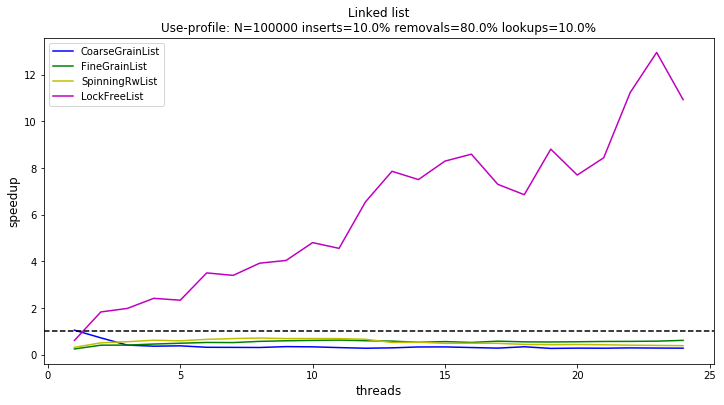
\includegraphics[width=1.0\linewidth]{figs/lateday/combined/lateday_combined_list_insert_10_lookup_10_removal_80}
\caption{Fig.}
\label{fig:fig1}
\end{figure}

\begin{figure}[h]
\centering
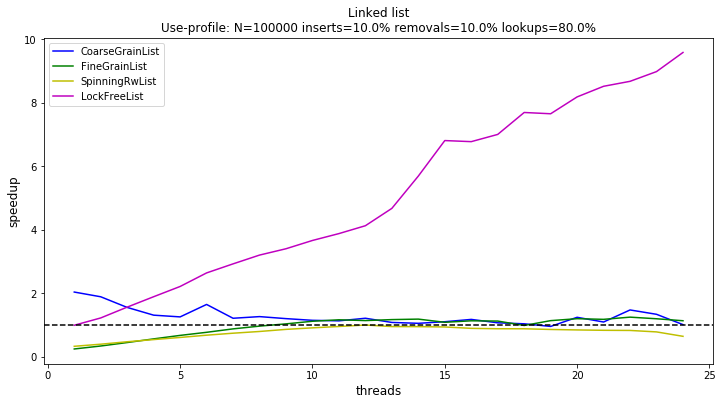
\includegraphics[width=1.0\linewidth]{figs/lateday/combined/lateday_combined_list_insert_10_lookup_80_removal_10}
\caption{Fig.}
\label{fig:fig1}
\end{figure}

\begin{figure}[h]
\centering
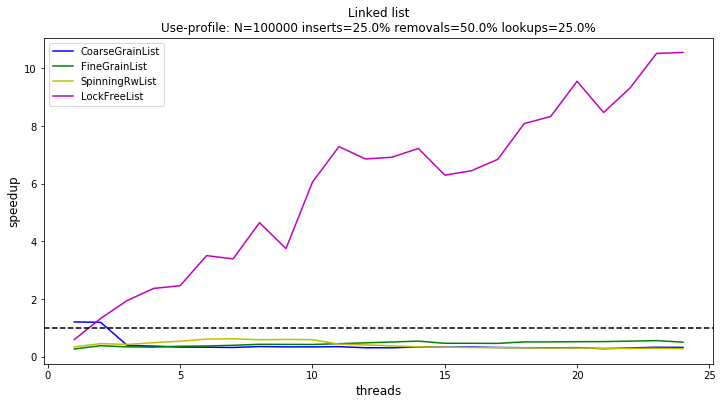
\includegraphics[width=1.0\linewidth]{figs/lateday/combined/lateday_combined_list_insert_25_lookup_25_removal_50}
\caption{Fig.}
\label{fig:fig1}
\end{figure}

\begin{figure}[h]
\centering
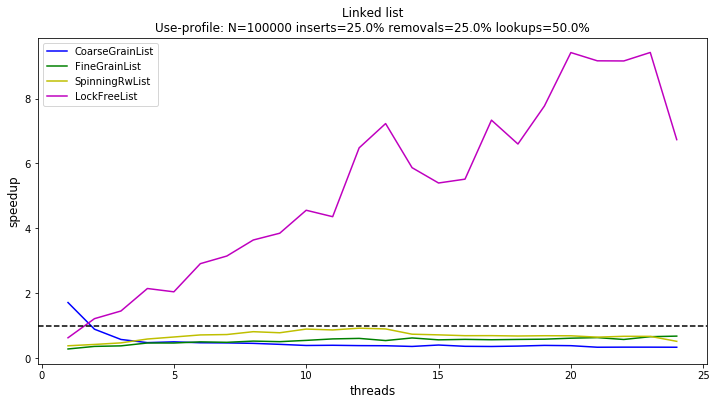
\includegraphics[width=1.0\linewidth]{figs/lateday/combined/lateday_combined_list_insert_25_lookup_50_removal_25}
\caption{Fig.}
\label{fig:fig1}
\end{figure}

\begin{figure}[h]
\centering
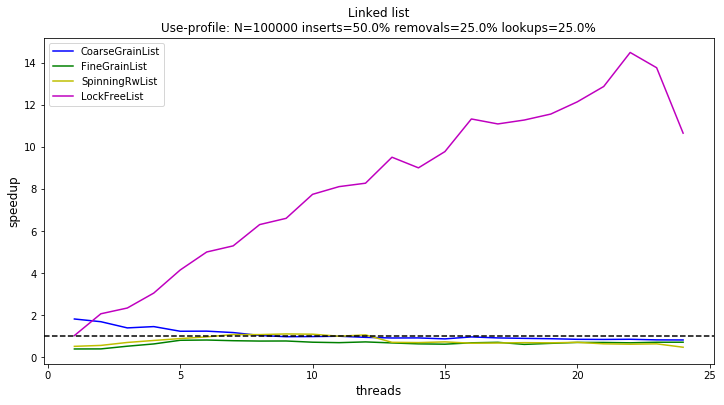
\includegraphics[width=1.0\linewidth]{figs/lateday/combined/lateday_combined_list_insert_50_lookup_25_removal_25}
\caption{Fig.}
\label{fig:fig1}
\end{figure}

\begin{figure}[h]
\centering
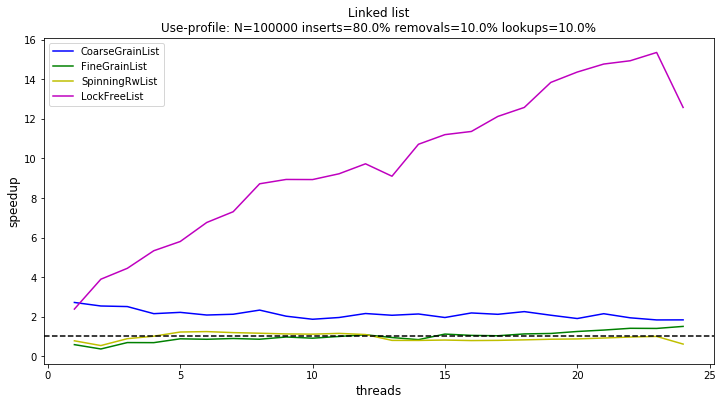
\includegraphics[width=1.0\linewidth]{figs/lateday/combined/lateday_combined_list_insert_80_lookup_10_removal_10}
\caption{Fig.}
\label{fig:fig1}
\end{figure}

\subsection{Hashmap results}

\begin{figure}[h]
\centering
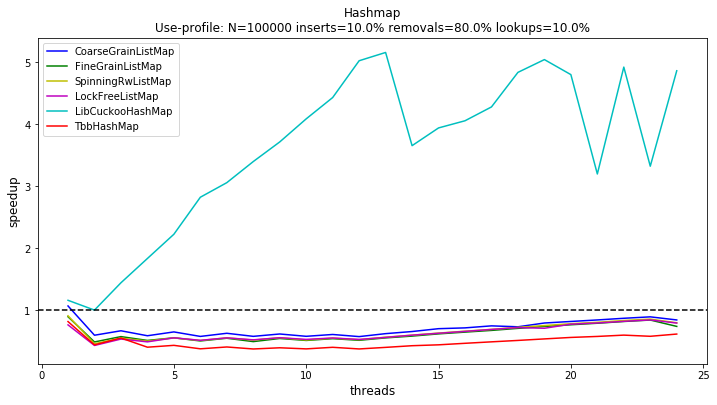
\includegraphics[width=0.5\linewidth]{figs/lateday/combined/lateday_combined_map_insert_10_lookup_10_removal_80}
\caption{Fig.}
\label{fig:fig2}
\end{figure}

\begin{figure}[h]
\centering
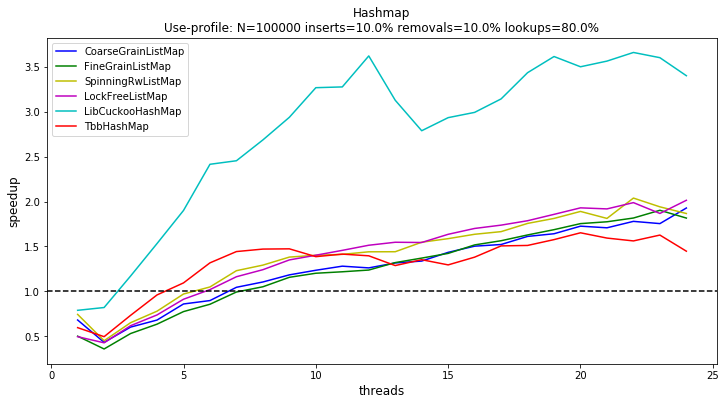
\includegraphics[width=0.5\linewidth]{figs/lateday/combined/lateday_combined_map_insert_10_lookup_80_removal_10}
\caption{Fig.}
\label{fig:fig2}
\end{figure}

\begin{figure}[h]
\centering
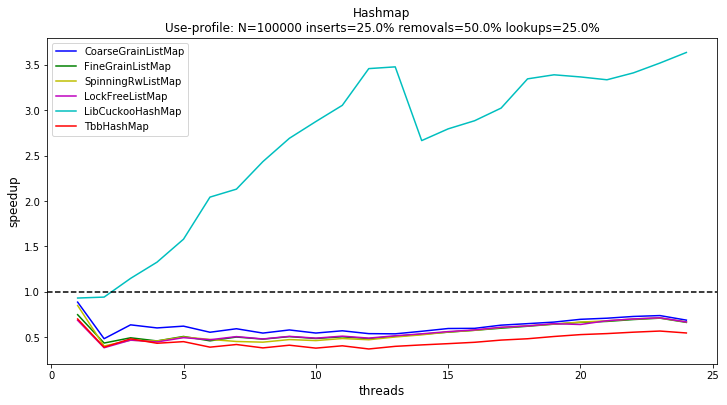
\includegraphics[width=0.5\linewidth]{figs/lateday/combined/lateday_combined_map_insert_25_lookup_25_removal_50}
\caption{Fig.}
\label{fig:fig2}
\end{figure}

\begin{figure}[h]
\centering
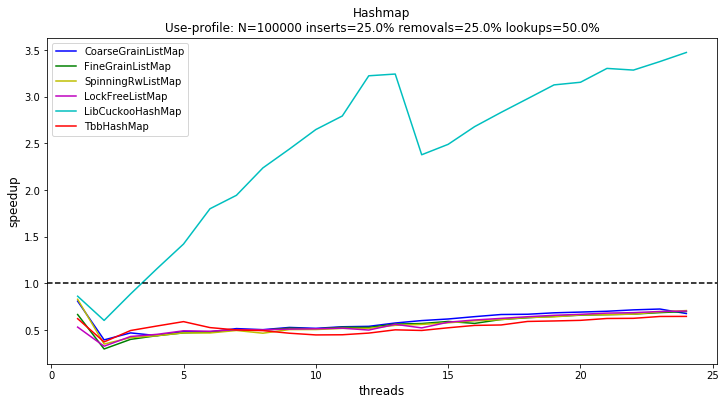
\includegraphics[width=0.5\linewidth]{figs/lateday/combined/lateday_combined_map_insert_25_lookup_50_removal_25}
\caption{Fig.}
\label{fig:fig2}
\end{figure}

\begin{figure}[h]
\centering
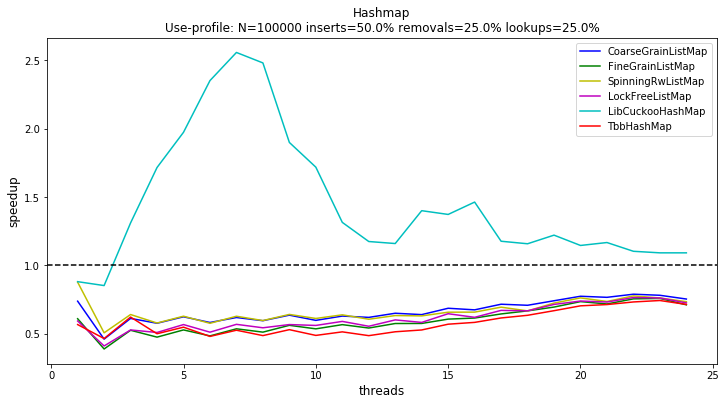
\includegraphics[width=0.5\linewidth]{figs/lateday/combined/lateday_combined_map_insert_50_lookup_25_removal_25}
\caption{Fig.}
\label{fig:fig2}
\end{figure}

\begin{figure}[h]
\centering
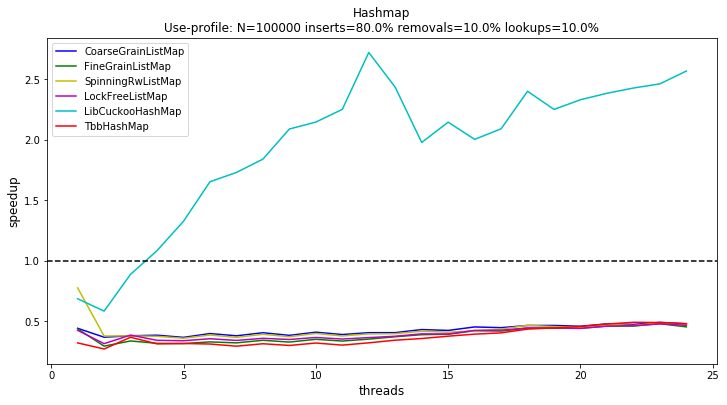
\includegraphics[width=0.5\linewidth]{figs/lateday/combined/lateday_combined_map_insert_80_lookup_10_removal_10}
\caption{Fig.}
\label{fig:fig2}
\end{figure}

\section{Conclusion}

\section{Division of Work}
Equal work was performed by both partners.

%lateday_combined_map_insert_10_lookup_10_removal_80.png
%lateday_combined_map_insert_10_lookup_80_removal_10.png
%lateday_combined_map_insert_25_lookup_25_removal_50.png
%lateday_combined_map_insert_25_lookup_50_removal_25.png
%lateday_combined_map_insert_50_lookup_25_removal_25.png
%lateday_combined_map_insert_80_lookup_10_removal_10.png



\printbibliography

\end{document}
\grid
